\documentclass{beamer}
%
% Choose how your presentation looks.
%
% For more themes, color themes and font themes, see:
% http://deic.uab.es/~iblanes/beamer_gallery/index_by_theme.html
%
\mode<presentation>
{
  \usetheme{default}      % or try Darmstadt, Madrid, Warsaw, ...
  \usecolortheme{default} % or try albatross, beaver, crane, ...
  \usefonttheme{default}  % or try serif, structurebold, ...
  \setbeamertemplate{navigation symbols}{}
  \setbeamertemplate{caption}[numbered]
} 
\usepackage{sansmathaccent}
\usepackage{xmpmulti}
\usepackage{movie15}
\pdfmapfile{+sansmathaccent.map}
\usepackage[english]{babel}
\usepackage[utf8x]{inputenc}

\usepackage{graphicx}

%\usepackage{animate}
\title[Your Short Title]{Exploration of chaos in shock waves}
\author{Jithin D. George}
%\institute{Where You're From}
%\date{Date of Presentation}
\AtBeginSection[]{\frame{\frametitle{Outline}%
		\usebeamerfont{myTOC}\tableofcontents[current]}}
\begin{document}

\begin{frame}
  \titlepage
\end{frame}

% Uncomment these lines for an automatically generated outline.
%\begin{frame}{Outline}
%  \tableofcontents
%\end{frame}

\section{Introduction}

\subsection{Background}
\begin{frame}{Background: Reactive Euler equations and detonation }

	\[\frac{D\rho}{Dt}=-\rho \nabla . u\]
	\[\rho\frac{Du}{Dt}=- \nabla P\]
	\[\rho\frac{D}{Dt}\bigg(h+\frac{|u|^2}{2}\bigg)=\frac{\partial P}{\partial t}\]
	\[\frac{DY_i}{Dt}=\dot{\omega_i}\]
	  \begin{center}
	  	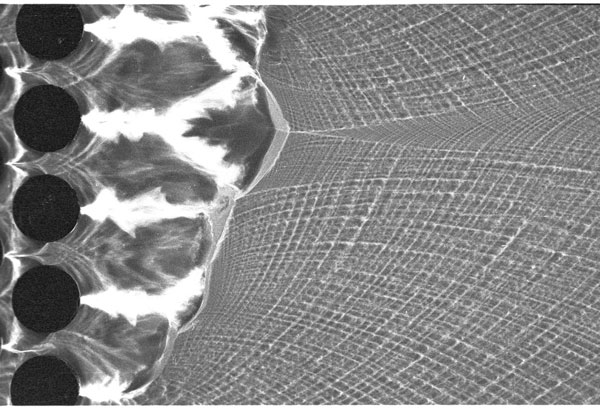
\includegraphics[height=100pt]{detonation}\\
	  	
	  \end{center}
\end{frame}	
\subsection{Model Equation}
\begin{frame}{Model Equation}


  \[u_t +\frac{1}{2}(u^2-uu_s)_x =f(x,u_s) \]

    \[x\in (-\infty,0)\]
    \[\textbf{Characteristic speed } = u-\frac{u_s}{2}\]

  






\end{frame}




	
\subsection{The nature of the source term}
\begin{frame}{The nature of the source term}
	\[f(x,u_{s})= \frac{q}{2\sqrt{4\pi \beta}} e^{-\frac{[x-x_f(u_s)]^2}{4\beta}}\]
	\[x_f(u_s) = \bigg(\frac{u_{0s}}{u_{s}}\bigg)^\alpha\]

  \begin{center}
  	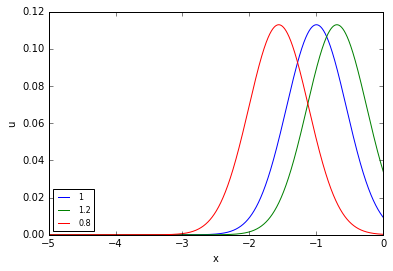
\includegraphics[height=150pt]{shiftinit}\\
  	
  \end{center}

\end{frame}	

\subsection{The Steady state solution}
\begin{frame}{The steady state solution}
	
	
	\[\frac{1}{2}(u_0^2-u_0u_{0s})' =f(x,u_{0s}) \]
	
	\[u_0(x)=\frac{u_{0s}}{2}+ \sqrt{2\int_{-\infty}^{x}f(y,u_{0s})dy}\]
	\[f= \frac{q}{2\sqrt{4\pi \beta}} e^{-\frac{[x-x_f(u_s)]^2}{4\beta}}\]
	\[u_0(x)= \frac{1}{2}\bigg[1+ \sqrt{\frac{1+erf((x+1)/2\sqrt{\beta})}{1+erf(1/2\sqrt{\beta})}}\bigg]\]
	
\end{frame}
	


\end{document}